%===================================== CHAP 3 =================================

\chapter{Project Management}

\section{Methodology}
\label{methodology}
During the development of the product the group decided to utilise scrum and the agile methodology. This was a natural choice of methodology as the customer required the process to be iterative and based on the group's previous experiences.

The process methodology was adjusted to suit the project in the best possible manner, as well as to suit the group's needs. The group completed daily meetings, sprint reviews and sprint retrospectives to achieve the best possible outcome of the project. The product owner of the project is also the project's customer, and will only be referred to as the customer throughout this document. To maintain consistent communication with the customer, there were scheduled stand-up meetings weekly or if needed. 

During the development process the group also utilised the principles of Extreme Programming, specifically the practice of pair programming. A decision based upon the groups desire to maximize the learning opportunities from each other resulting in the best possible outcome. 

\subsection{Development}
Throughout the development the group utilised the practice of issue tracking on GitHub (see \ref{GitHub}), and structured the tasks based on a roadmap using milestones. To ensure that the group followed the principles of scrum, it was decided to define the milestones as a correspondence to time.

To easily track the issues during the development the group used waffle.io (see \ref{Waffle.io}) as a scrum board. This provided the group a visualisation of the process, with issues in 'product backlog', 'sprint backlog' and 'in process' including who is working on which, using assignees. 

\subsection{Report}
Waffle.io (see \ref{Waffle.io}) was also used during the process of writing the report, primarily to ensure that every member participated in writing the report, and every member needed to proof-read each part before it were categorized as done.

\section{Team Organization}\label{projectOrganisation}
The group decided to divide the project into reasonable areas and delegate the main responsibility to two or three of the group members, where one had the primary responsibility. This would ensure that all parts of the project were kept in mind during the development, as well as more than one person knew what was going on in one specific area.

\subsubsection{Scrum Master}
Responsible: Ingrid Skar \\
Skar was given the role as Scrum Master due to previous experience with leading a team and the coordination of scrum related tasks. This includes coordinating workpackages, sprints and milestones.

\subsubsection{Group Leader}
Responsible: Christina Hellenes Andresen \\
Andresen was voted to the role as group leader, this includes attending group leader meetings. The group also decided that the group leader was to create meeting agendas and lead the group meetings. 

\subsubsection{Contact Responsible}
Responsible: Sigve André Evensen Skaugvoll \\
The responsible person for keeping contact with both customer and supervisor was Skaugvoll. He was responsible of arranging meetings and sending them the meeting agenda before meetings.

\subsubsection{Architect}
Responsible: Martin Stigen \\
The role of architect was given to Stigen, due to interests and experience. The architect was responsible for providing initial draft to the architecture and for integrating the back end together with the front end. Skaugvoll was also a part of the architect team.

\subsubsection{Database}
Responsible: Andreas Norstein\\
Norstein was given the main responsibility for the database, this responsibility contains investigating the different options and needs. Norstein had this responsibility together with Skaugvoll.

\subsubsection{Back End}
Responsible: Sigve André Evensen Skaugvoll\\
The back end responsible was responsible for investigation the back end options. Norstein worked together with Skaugvoll after the group had decided on using Django to set up the development environment. Skaugvoll and Norstein were elected based on some prior experience through own projects, course at NTNU and interests.

\subsubsection{Front End}
Responsible: Thomas Wold\\
Wold was given the role of front end responsible, this were mainly because of experiences with front end development from courses he had attended at NTNU. This responsibility was shared with Skar and Stigen. Their work included choosing development language, framework and libraries, as well as preparing the development environment.

\subsubsection{Graphical User Interface Designer}
Responsible: Ingrid Skar\\
The graphical user interface designer was responsible for creating the paper prototype and styling the product. Skar was given the main responsibility to this task, together with Andresen, mainly because of interests in this field.

\subsubsection{Testing}
Responsible: Sigve André Evensen Skaugvoll\\
Skaugvoll was given the role as tester, this includes to set up test strategy and plan. Andresen and Skar were co-responsible for testing. 

\subsubsection{Report}
Responsible: Christina Hellenes Andresen\\
Andresen was given the role of report responsible, due to previous experience. This role includes setting up the table of content and keeping the report backlog on Waffle.io, \ref{Waffle.io}, updated. Wold was also a part of this team.


\section{Work Breakdown Structure}
The group decided to break down the project key activities into manageable sections, defined as work packages (see fig. \ref{Work_Breakdown_Structure}). By outlining the project and organizing it into smaller sections the group achieved a greater understanding of the scope of what was expected to be developed. The work breakdown structure outlined the project, providing the group further definition and description of the what was included in the work packages. 

\begin{figure}[h!]
\centering
    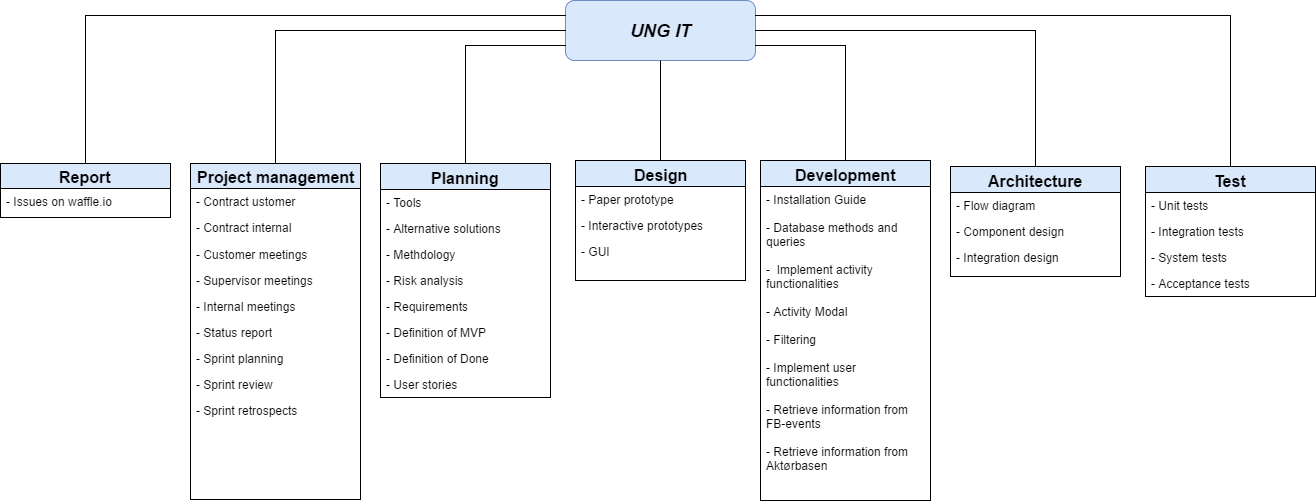
\includegraphics[width=1\textwidth]{fig/work_packages}
\caption{Work Breakdown Structure}
\label{Work_Breakdown_Structure}
\end{figure}

\subsection{Gantt Diagram} 
The project's life cycle was visualised using a Gantt Diagram (see fig. \ref{Gantt_Diagram}) . This was useful while planning the development process, as the group achieved a common understanding of how long each phase of the project should be, and determine resources based on this. 

As the project was to be developed according to agile methodologies (see \ref{methodology}) the model reflects this. The development is divided into iterations, sprints, lasting 2 weeks. The life cycle of the Other work packages depended on the scope; some lasted throughout the entire project, such as project management, and others occurred in specific phases, such as planning or testing. 

\begin{figure}[h!]
\centering
    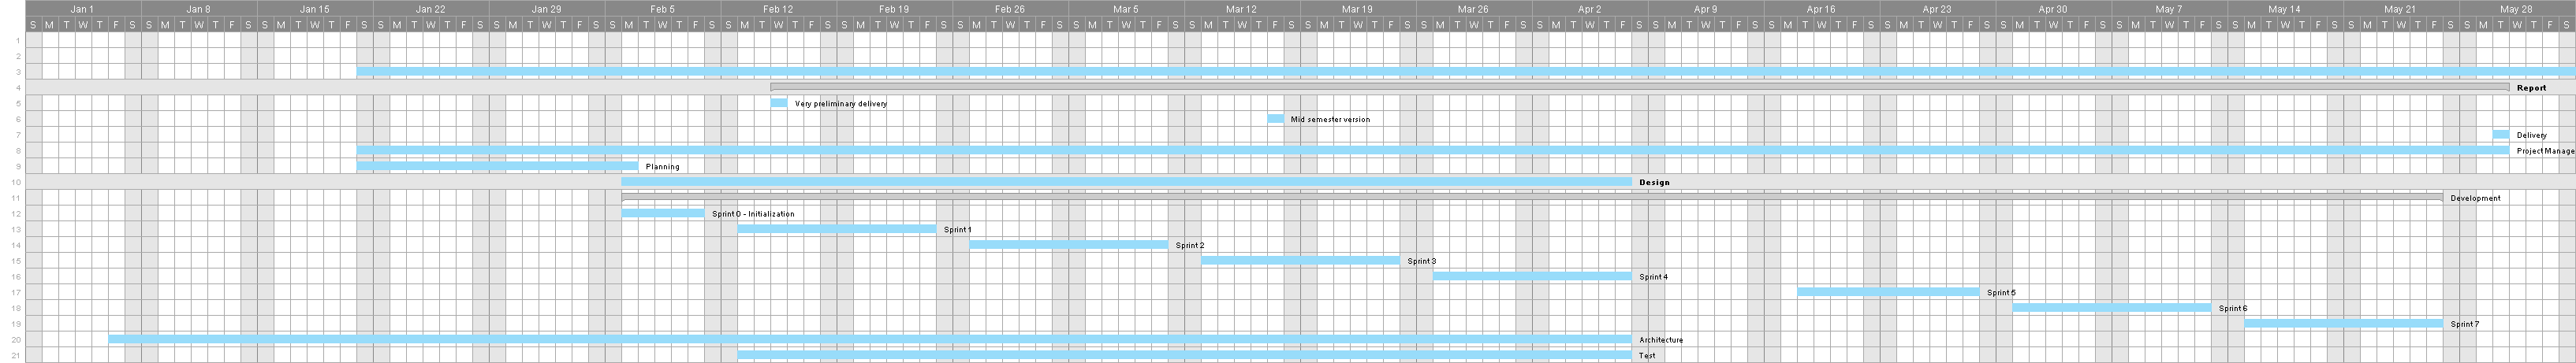
\includegraphics[width=1.0\textwidth]{fig/gantt}
\caption{Gantt Diagram}
\label{Gantt_Diagram}
\end{figure}

\section{Risk Analysis} 
\label{riskAnalysis}
The initial risk analysis (see table \ref{risk_analysis}) was created during sprint iteration 0. The cases and their values were mainly based on previous experience from other projects. During the development of the project they were adapted to by thoroughly going through each case collaboratively, doing new evaluations. The updated risk analysis can be found in section \ref{updated_risk_analysis} 

Each risk were evaluated and given a number between 1 and 9. Where one is minimal likelihood, but may occur and 9 is very likely to occur. The group then arrange the risks according to importance and sorted the risks in deciding order. The preventive actions are actions the group will preform to prevent the risk of happening. If a risk occurs the group should look at the remedial action to know what action to perform. 


\begin{longtable}{@{\extracolsep{\fill}}
                |L{0.14\linewidth}
                |L{0.09\linewidth}
                |L{0.09\linewidth}
                |L{0.14\linewidth}
                |L{0.17\linewidth}
                |L{0.17\linewidth}|@{}}
\hline


\rowcolor{Gray}
\textbf{Description} & \textbf{Likelihood (1-9)} & \textbf{ Impact (1-9)} & \textbf{Importance {\footnotesize (Likelihood * Impact)}} & \textbf{Preventive Action}    & \textbf{Remedial Action} \\ \hline


Conflicts in group & 7 & 7 & 49 & Talk together, give constructive feedback & Try to resolve it with a neutral third party \\
\hline
Unrealistic goals & 7 & 6 & 42 & Talk to customer, be realistic & Be flexible and change goals \\
\hline
Falling Behind Schedule & 6 & 6 & 36 & Daily stand-up meetings, be efficient at meetings, have scheduled meetings & Re-estimate workload, increase work hours \\
\hline
Sickness & 8 & 4 & 32 & Eat healthy, be hygienic & Stay at home, if possible work from home \\
\hline
Technical challenges & 5 & 6 & 30 & Think ahead, test early, build modular & Reconsider technical choices, contact people with knowledge \\
\hline
Lack of knowledge & 9 & 3 & 27 & Be prepared, read up on topic/tech & Ask for help, read about the topics we miss knowledge about \\
\hline
Merge conflicts & 8 & 3 & 24 & Always pull from master before branching & Solve it, run unit tests after resolving conflict \\
\hline
Absent customer & 3 & 7 & 21 & Have scheduled meetings & Refer to customer contract \\
\hline
Lack of communication in group & 5 & 4 & 20 & Slack and meetings & Talk to group representative \\
\hline
Lack of responsibility & 3 & 6 & 18 & Daily stand-up meetings, follow up on given tasks, collaborative work hours & Group leader’s responsibility to follow up \\
\hline
Inefficient meetings & 8 & 2 & 16 & Follow the agenda for the meeting, strict group leader, bring coffee & Take breaks \\
\hline
Late Arrivals & 8 & 2 & 16 & Give reminders, use the calendar & Cake punishment, contact supervisor if it repeats \\
\hline
Data loss & 2 & 6 & 12 & Save often, use git, commit and push often, have local copies & Increase workload, redo work \\
\hline
Poor execution of methodology & 4 & 3 & 12 & Strict group leader, scrum master, quick recap of methodology & Recap of methodology \\
\hline
Absence & 2 & 5 & 10 & Give reminders, use the calendar & Cake punishment, contact supervisor if it repeats \\
\hline
Disagreement of priorities & 5 & 2 & 10 & Everyone gets the opportunity to say what they mean & Talk to customer \\
\hline
Loss of group members & 1 & 9 & 9 & Group representative, social activities & Distribute workload equally over the entire team, adjust goals of project \\
\hline

\caption{Risk Analysis}
\label{risk_analysis}
\end{longtable}



\section{Sprints}
\label{sprintsAndMilestones}
The group divided the development process into sprints (see table \ref{Sprints}), were each sprint lasted for two weeks running Monday to Friday the next week, and planned with respect to the given milestones (see \ref{milestones}). During the sprints the group arranged daily stand-up meetings (see \ref{daily-meetings}) and workdays (see \ref{workdays}) to plan and work on the project. At the end of each sprint, sprint retrospects where held. Each member evaluated how the group had collaborated during the just completed sprint, and determined actions to make the upcoming sprint more productive.

\begin{longtable}{@{\extracolsep{\fill}}
                |L{0.16\linewidth}
                |L{0.18\linewidth}
                |L{0.12\linewidth}
                |L{0.40\linewidth}|@{}}
               
\hline
\rowcolor{Gray}
\textbf{Dates}&\textbf{Planned Work Hours}&\textbf{Sprint}&\textbf{Goal}\\
\hline
06.02 - 10.02&136.5&Sprint 0&Initialization phase. Planning, product backlog set up and first draft design.\\
\hline
13.02 - 24.02&270&Sprint 1& Deliver first interactive prototype to customer, this includes the routing to different pages and the page with overview of events.\\
\hline
27.02 - 10.03&270&Sprint 2& The sprint goal is implement functionality on the activities page; allowing the user to create and retrieve events, as well as filter these.\\
\hline
13.03 - 24.03&270&Sprint 3&-\\
\hline
27.03 - 07.04&270&Sprint 4&-\\
\hline
18.04 - 28.04&270&Sprint 5&Find and fix bugs.\\
\hline
01.05 - 30.05&360&Sprint 6&Final touch report, first aid kit and deliver\\
\hline
\caption{Sprints}
\label{Sprints}
\end{longtable}


\subsection{Workdays}
\label{workdays}
The group had four workdays a week (see table \ref{Time table}). The working hours were decided in the planning phase. During these hours it was expected that every member sat together and worked on the project. The hours were sat at times were no one had lectures or other activities to attend. To sit together and work made it easier to have an overview of what the rest of the group were working on and to get help from each other. During the workdays the group members worked on individual tasks.

\subsection{Daily Meetings}
\label{daily-meetings}
The daily meetings lasted for 15 minutes, and were used to update each other on what tasks each member was working on, any problems and agree on different decisions. Mondays was used to plan the upcoming sprint or review the progress of the ongoing sprint. The daily meetings were all documented (see example in appendix \ref{meeting_minutes_daily_meetings})


\begin{longtable}{@{\extracolsep{\fill}}
                |L{0.15\linewidth}
                |L{0.12\linewidth}
                |L{0.14\linewidth}
                |L{0.14\linewidth}
                |L{0.12\linewidth}
                |L{0.12\linewidth}|@{}}
\hline
\rowcolor{Gray}
&\textbf{Monday} & \textbf{Tuesday} & \textbf{Wednesday} & \textbf{Thursday} & \textbf{Friday} \\
\hline
08:15 - 09:00 & & & Meeting & & \\
\hline
09:15 - 10:00 & & & Customer meeting & & \\
\hline
10:15 - 11:00 & & Meeting & Workday & Meeting & Meeting \\
\hline
11:15 - 12:00 & & Bi-weekly supervisor meeting & Workday & Workday & Workday \\
\hline
12:15 - 13:00 & & Workday & Workday & Workday & Workday \\
\hline
13:15 - 14:00 & & Workday & Workday       & Workday       & Workday       \\
\hline
14:15 - 15:00 & Meeting &               & Workday       &               & Workday       \\
\hline
15:15 - 16:00 & Meeting &               & Workday       &               & Workday\\
\hline
\caption{Weekly Time Table}
\label{Time table}
\end{longtable}


\subsection{Customer Meetings}
Initially, the customer and the group decided to meet bi-weekly, but realised this was too infrequent as the project developed. This was resolved by arranging weekly meetings. During these meetings the group updated the customer on the project status, demonstrated latest prototype and got feedback on what tasks to prioritize next. This ensured that the product developed corresponded to customer's vision. All meetings with the customer were documented (see example in appendix \ref{meeting_minutes_customer_meetings}).
 
\subsection{Supervisor Meetings}
The group met with the supervisor bi-weekly. During these meetings the supervisor was updated on the work completed and the plan for the next weeks. The supervisor also supported the group by answering questions regarding the report, work process and other relevant questions. All meetings were documented and the meeting minutes were sent to the supervisor's after the meeting (see example in appendix \ref{meeting_minutes_supervisor_meetings}).


\section{Milestones}
\label{milestones}
The milestones (see table \ref{Milestones}) are the important dates given in the project and an internal deadline. In addition to this, the milestones consist of the project's phases - in accordance to GitHub's guidelines \cite{GitHubGuide}. The milestones related to the product included issues (see \ref{product_backlog}), which were mainly based on the user stories (see \ref{User Stories}). They were created as the project evolved together with the customer. 

\begin{longtable}{@{\extracolsep{\fill}}
                |L{0.10\linewidth}
                |L{0.15\linewidth}
                |L{0.65\linewidth}|@{}}
\hline
\rowcolor{Gray}
\textbf{Date} & \textbf{Milestone} & \textbf{Description} \\
\hline
10.02 & Milestone 0 & Create first design draft, plan and set up preliminary version of product backlog and set up development environment \\
\hline
15.02 & Report & Very preliminary delivery of report \\
\hline
24.02 & Milestone 1 & Create skeleton of product, create database with activities and begin with possibility of log in with different roles. \\
\hline
03.03 & Milestone 2 & Create and retrieve new events. \\
\hline
17.03 & Milestone 3 & Should be possible to sign up for an activity, filter activities and the installation guide should be made. \\
\hline
19.03 & Report & Mid semester version of report\\
\hline
24.03 & Milestone 4 & User testing \\
\hline
07.04 & Milestone 5 & Group deadline. No new features should be implemented. \\
\hline
Week 19 & & Final Presentation \\
\hline
30.05 &  & Deliver  \\
\hline
\caption{Milestones}
\label{Milestones}
\end{longtable}

\subsection{Product Backlog}
\label{product_backlog}
The product backlog were requested by the customer to be updated as the product evolved. This were to be done on GitHub (see \ref{GitHub}), so the customer had all necessary information in one place (see fig. \ref{Open Issues} and fig. \ref{Closed Issues}). The group used Waffle.io (see \ref{Waffle.io}) to manage the product backlog, with labels which indicated the related user story (see \ref{User Stories}) and the development status.


\begin{figure}[h!]
\centering
    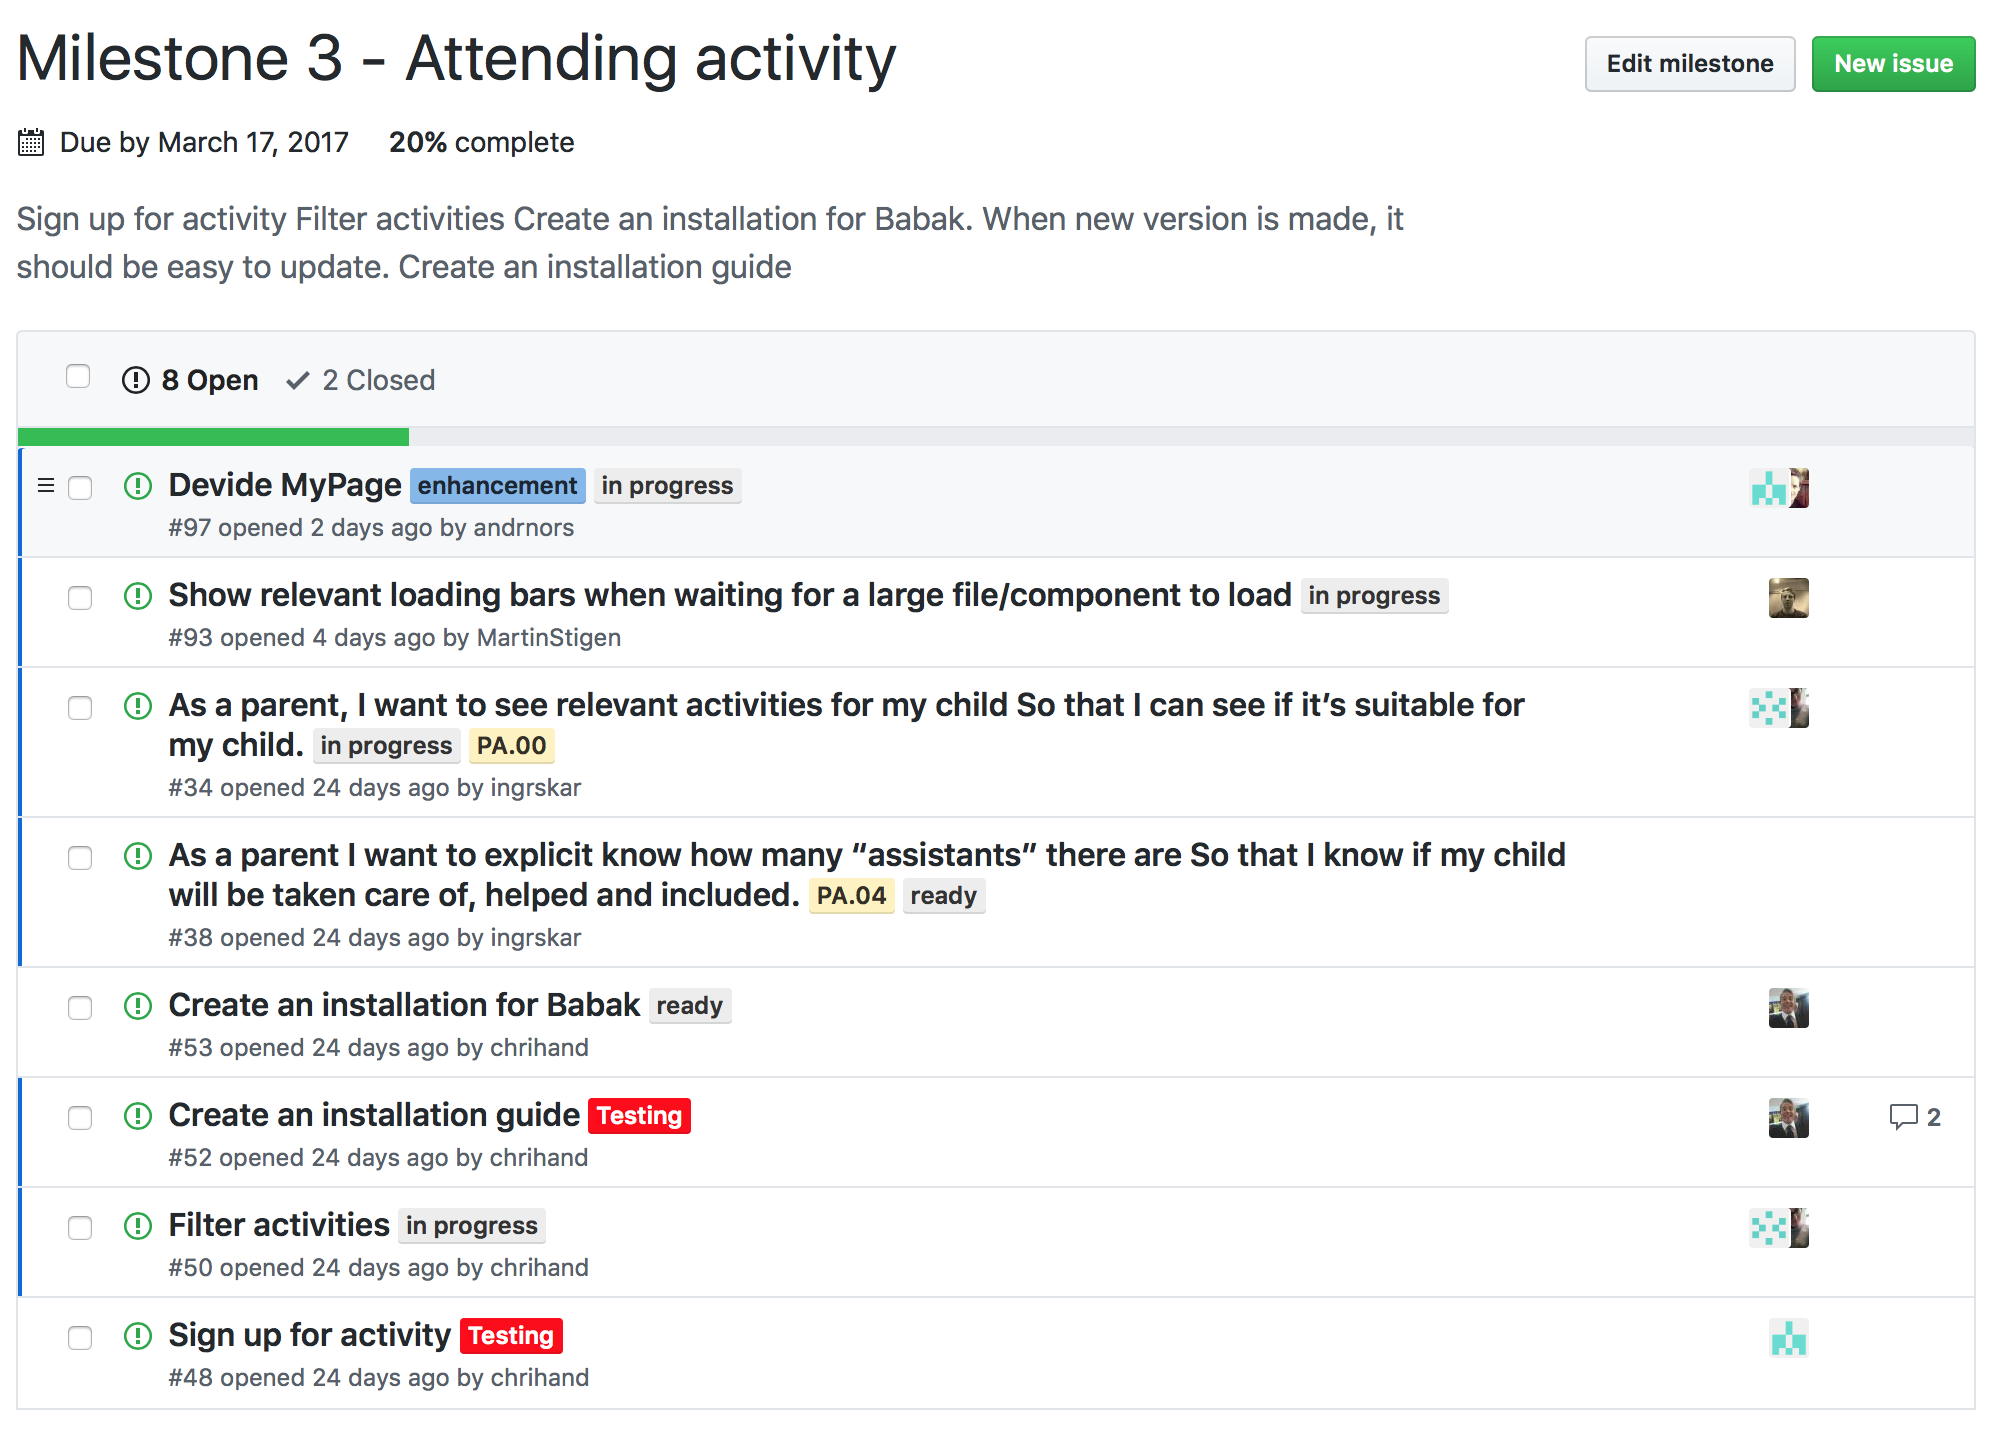
\includegraphics[width=0.7\textwidth]{fig/open_issues}
\caption{Milestone 3, open issues}
\label{Open Issues}
\end{figure}

\begin{figure}[h!]
\centering
    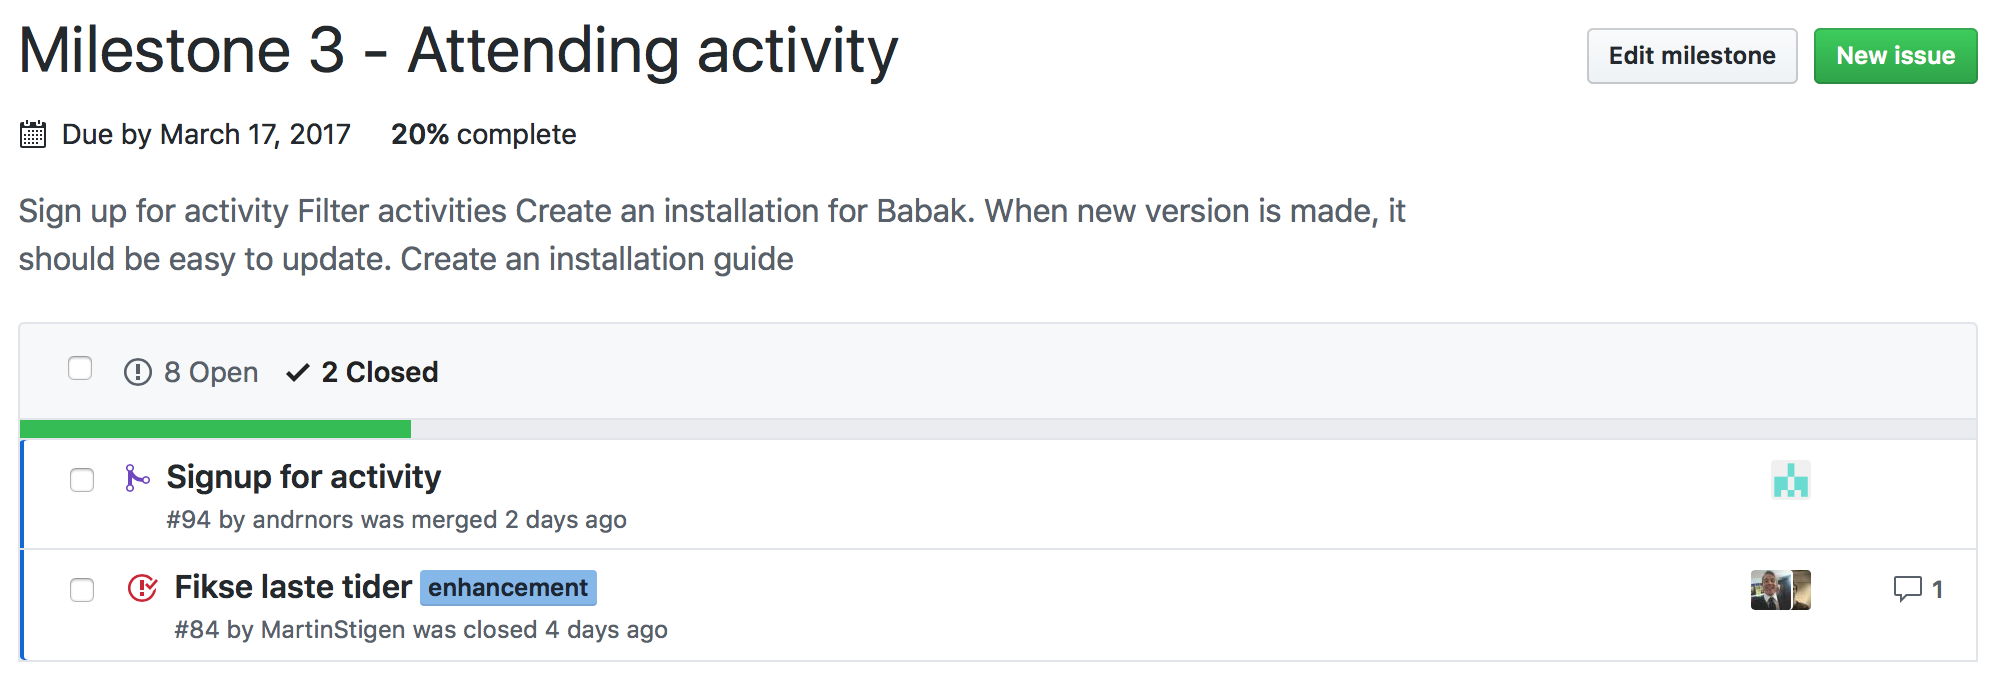
\includegraphics[width=0.7\textwidth]{fig/closed_issues}
\caption{Milestone 3, closed issues}
\label{Closed Issues}
\end{figure}


\cleardoublepage